\documentclass[10pt,a4paper,oneside,fleqn]{article}
\usepackage{geometry}
\geometry{a4paper,left=20mm,right=20mm,top=1cm,bottom=2cm}
\usepackage[utf8]{inputenc}
%\usepackage{ngerman}
\usepackage{amsmath}                % brauche ich um dir Formel zu umrahmen.
\usepackage{amsfonts}                % brauche ich für die Mengensymbole
\usepackage{graphicx}
\setlength{\parindent}{0px}
\setlength{\mathindent}{10mm}
\usepackage{bbold}                    %brauche ich für die doppel Zahlen Darstellung (Einheitsmatrix z.B)



\usepackage{color}
\usepackage{titlesec} %sudo apt-get install texlive-latex-extra

\definecolor{darkblue}{rgb}{0.1,0.1,0.55}
\definecolor{verydarkblue}{rgb}{0.1,0.1,0.35}
\definecolor{darkred}{rgb}{0.55,0.2,0.2}

%hyperref Link color
\usepackage[colorlinks=true,
        linkcolor=darkblue,
        citecolor=darkblue,
        filecolor=darkblue,
        pagecolor=darkblue,
        urlcolor=darkblue,
        bookmarks=true,
        bookmarksopen=true,
        bookmarksopenlevel=3,
        plainpages=false,
        pdfpagelabels=true]{hyperref}

\titleformat{\chapter}[display]{\color{darkred}\normalfont\huge\bfseries}{\chaptertitlename\
\thechapter}{20pt}{\Huge}

\titleformat{\section}{\color{darkblue}\normalfont\Large\bfseries}{\thesection}{1em}{}
\titleformat{\subsection}{\color{verydarkblue}\normalfont\large\bfseries}{\thesubsection}{1em}{}

% Notiz Box
\usepackage{fancybox}
\newcommand{\notiz}[1]{\vspace{5mm}\ovalbox{\begin{minipage}{1\textwidth}#1\end{minipage}}\vspace{5mm}}

\usepackage{cancel}
\setcounter{secnumdepth}{3}
\setcounter{tocdepth}{3}





%-------------------------------------------------------------------------------
%Diff-Makro:
%Das Diff-Makro stellt einen Differentialoperator da.
%
%Benutzung:
% \diff  ->  d
% \diff f  ->  df
% \diff^2 f  ->  d^2 f
% \diff_x  ->  d/dx
% \diff^2_x  ->  d^2/dx^2
% \diff f_x  ->  df/dx
% \diff^2 f_x  ->  d^2f/dx^2
% \diff^2{f(x^5)}_x  ->  d^2(f(x^5))/dx^2
%
%Ersetzt man \diff durch \pdiff, so wird der partieller
%Differentialoperator dargestellt.
%
\makeatletter
\def\diff@n^#1{\@ifnextchar{_}{\diff@n@d^#1}{\diff@n@fun^#1}}
\def\diff@n@d^#1_#2{\frac{\textrm{d}^#1}{\textrm{d}#2^#1}}
\def\diff@n@fun^#1#2{\@ifnextchar{_}{\diff@n@fun@d^#1#2}{\textrm{d}^#1#2}}
\def\diff@n@fun@d^#1#2_#3{\frac{\textrm{d}^#1 #2}{\textrm{d}#3^#1}}
\def\diff@one@d_#1{\frac{\textrm{d}}{\textrm{d}#1}}
\def\diff@one@fun#1{\@ifnextchar{_}{\diff@one@fun@d #1}{\textrm{d}#1}}
\def\diff@one@fun@d#1_#2{\frac{\textrm{d}#1}{\textrm{d}#2}}
\newcommand*{\diff}{\@ifnextchar{^}{\diff@n}
  {\@ifnextchar{_}{\diff@one@d}{\diff@one@fun}}}
%
%Partieller Diff-Operator.
\def\pdiff@n^#1{\@ifnextchar{_}{\pdiff@n@d^#1}{\pdiff@n@fun^#1}}
\def\pdiff@n@d^#1_#2{\frac{\partial^#1}{\partial#2^#1}}
\def\pdiff@n@fun^#1#2{\@ifnextchar{_}{\pdiff@n@fun@d^#1#2}{\partial^#1#2}}
\def\pdiff@n@fun@d^#1#2_#3{\frac{\partial^#1 #2}{\partial#3^#1}}
\def\pdiff@one@d_#1{\frac{\partial}{\partial #1}}
\def\pdiff@one@fun#1{\@ifnextchar{_}{\pdiff@one@fun@d #1}{\partial#1}}
\def\pdiff@one@fun@d#1_#2{\frac{\partial#1}{\partial#2}}
\newcommand*{\pdiff}{\@ifnextchar{^}{\pdiff@n}
  {\@ifnextchar{_}{\pdiff@one@d}{\pdiff@one@fun}}}
\makeatother
%
%Das gleich nur mit etwas andere Syntax. Die Potenz der Differentiation wird erst
%zum Schluss angegeben. Somit lautet die Syntax:
%
% \diff_x^2  ->  d^2/dx^2
% \diff f_x^2  ->  d^2f/dx^2
% \diff{f(x^5)}_x^2  ->  d^2(f(x^5))/dx^2
% Ansonsten wie Oben.
%
%Ersetzt man \diff durch \pdiff, so wird der partieller
%Differentialoperator dargestellt.
%
%\makeatletter
%\def\diff@#1{\@ifnextchar{_}{\diff@fun#1}{\textrm{d} #1}}
%\def\diff@one_#1{\@ifnextchar{^}{\diff@n{#1}}%
%  {\frac{\textrm d}{\textrm{d} #1}}}
%\def\diff@fun#1_#2{\@ifnextchar{^}{\diff@fun@n#1_#2}%
%  {\frac{\textrm d #1}{\textrm{d} #2}}}
%\def\diff@n#1^#2{\frac{\textrm d^#2}{\textrm{d}#1^#2}}
%\def\diff@fun@n#1_#2^#3{\frac{\textrm d^#3 #1}%
%  {\textrm{d}#2^#3}}
%\def\diff{\@ifnextchar{_}{\diff@one}{\diff@}}
%\newcommand*{\diff}{\@ifnextchar{_}{\diff@one}{\diff@}}
%
%Partieller Diff-Operator.
%\def\pdiff@#1{\@ifnextchar{_}{\pdiff@fun#1}{\partial #1}}
%\def\pdiff@one_#1{\@ifnextchar{^}{\pdiff@n{#1}}%
%  {\frac{\partial}{\partial #1}}}
%\def\pdiff@fun#1_#2{\@ifnextchar{^}{\pdiff@fun@n#1_#2}%
%  {\frac{\partial #1}{\partial #2}}}
%\def\pdiff@n#1^#2{\frac{\partial^#2}{\partial #1^#2}}
%\def\pdiff@fun@n#1_#2^#3{\frac{\partial^#3 #1}%
%  {\partial #2^#3}}
%\newcommand*{\pdiff}{\@ifnextchar{_}{\pdiff@one}{\pdiff@}}
%\makeatother

%-------------------------------------------------------------------------------
%%Nützliche Makros um in der Quantenmechanik Bras, Kets und das Skalarprodukt
%%zwischen den beiden darzustellen.
%%Benutzung:
%% \bra{x}  ->    < x |
%% \ket{x}  ->    | x >
%% \braket{x}{y} ->   < x | y >

\newcommand\bra[1]{\left\langle #1 \right|}
\newcommand\ket[1]{\left| #1 \right\rangle}
\newcommand\braket[2]{%
  \left\langle #1\vphantom{#2} \right.%
  \left|\vphantom{#1#2}\right.%
  \left. \vphantom{#1}#2 \right\rangle}%

%-------------------------------------------------------------------------------
%%Aus dem Buch:
%%Titel:  Latex in Naturwissenschaften und Mathematik
%%Autor:  Herbert Voß
%%Verlag: Franzis Verlag, 2006
%%ISBN:   3772374190, 9783772374197
%%
%%Hier werden drei Makros definiert:\mathllap, \mathclap und \mathrlap, welche
%%analog zu den aus Latex bekannten \rlap und \llap arbeiten, d.h. selbst
%%keinerlei horizontalen Platz benötigen, aber dennoch zentriert zum aktuellen
%%Punkt erscheinen.

\newcommand*\mathllap{\mathstrut\mathpalette\mathllapinternal}
\newcommand*\mathllapinternal[2]{\llap{$\mathsurround=0pt#1{#2}$}}
\newcommand*\clap[1]{\hbox to 0pt{\hss#1\hss}}
\newcommand*\mathclap{\mathpalette\mathclapinternal}
\newcommand*\mathclapinternal[2]{\clap{$\mathsurround=0pt#1{#2}$}}
\newcommand*\mathrlap{\mathpalette\mathrlapinternal}
\newcommand*\mathrlapinternal[2]{\rlap{$\mathsurround=0pt#1{#2}$}}

%%Das Gleiche nur mit \def statt \newcommand.
%\def\mathllap{\mathpalette\mathllapinternal}
%\def\mathllapinternal#1#2{%
%  \llap{$\mathsurround=0pt#1{#2}$}% $
%}
%\def\clap#1{\hbox to 0pt{\hss#1\hss}}
%\def\mathclap{\mathpalette\mathclapinternal}
%\def\mathclapinternal#1#2{%
%  \clap{$\mathsurround=0pt#1{#2}$}%
%}
%\def\mathrlap{\mathpalette\mathrlapinternal}
%\def\mathrlapinternal#1#2{%
%  \rlap{$\mathsurround=0pt#1{#2}$}% $
%}

%-------------------------------------------------------------------------------
%%Hier werden zwei neue Makros definiert \overbr und \underbr welche analog zu
%%\overbrace und \underbrace funktionieren jedoch die Gleichung nicht
%%'zerreißen'. Dies wird ermöglicht durch das \mathclap Makro.

\def\overbr#1^#2{\overbrace{#1}^{\mathclap{#2}}}
\def\underbr#1_#2{\underbrace{#1}_{\mathclap{#2}}}


\begin{document}

\textit{29. März 2012}
\input{../headers/authors.tex}
\setcounter{section}{1}
\section*{Doppelmuldenpotential}


\begin{figure}[htbp]
  \centering
  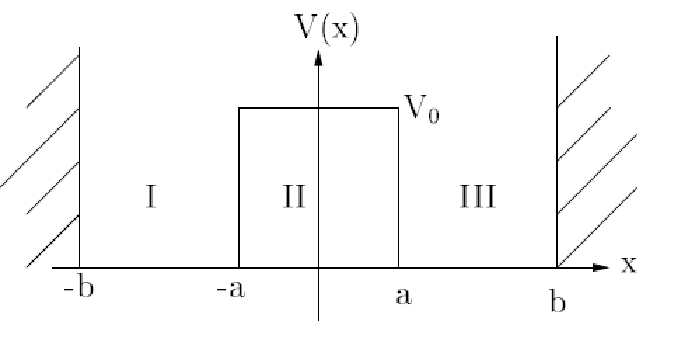
\includegraphics{./sgl_doppelmuldenpotential_pics/pic01_v.pdf}
  \caption{Doppelmuldenpotential}
  \label{fig:fg1}
\end{figure}

Beim Doppelmuldenpotential interessiert uns vorwiegend ein Teilchen welches eine Energie kleiner als der mittlere Potentialkasten hat. Wie man später aus der Rechnung ersieht, gibt es zwei mögliche Lösungen (positive/negative Parität) für das Problem. Da Superposition der beiden Lösungen wieder eine ergibt, stellt man fest, dass nach Summieren der beiden Lösungen die Wellenfunktion vollständig nur im Bereich I existiert. Zieht man dagegen die beiden Lösungen voneinander ab, so ist die Welle nur in Bereich III vorzufinden. Dieses Verhalten wird als \textbf{tunneln} des Teilchens interpretiert.\\
\\
Wir werden die supperpositionierte Lösung auch zeitentwickeln und eine \textbf{Tunnelzeit} feststellen. Ein Beispiel für dieses Phänomen ist das Ammoniakmolekül. Hierbei tunnelt das Stickstoffatom durch die Ebene dreier Wasserstoffatome. Seine Schwinungsfrequenz beträgt (laut wiki) 23,786 GHz.


\section*{Allgemeiner Ansatz}

\begin{equation}
  \label{eq:1}
  \psi_I = Ae^{ikx}+Be^{-ikx} \qquad \text{mit } k = \sqrt{\frac{2m}{\hbar}E}
\end{equation}

\begin{equation}
  \label{eq:2}
  \psi_{II} = Ce^{q x}+De^{-qx}\qquad \text{mit } q = \sqrt{\frac{2m}{\hbar}(V-E)}
\end{equation}

\begin{equation}
  \label{eq:3}
  \psi_{III} = Fe^{ikx}+Ge^{-ikx}\qquad \text{mit (siehe }\psi_{I}) k = \sqrt{\frac{2m}{\hbar}E}
\end{equation}


Die Randbedingung besagt, dass die Wellenfuktion am Rand des unendlichen  Potentials verschwindet. Das kann man für eine Konkretisierung von Teilbereich I und III ausnutzen:

\begin{align}
  \label{eq:4}
  \psi_{I}(-b) &= 0 = Ae^{-ikb}+Be^{ikb} \notag \\
\Leftrightarrow & A = -Be^{2ikb}\qquad\text{A in }\ref{eq:1}\text{ einsetzen} \notag\\
\psi_I(x)&=-Be^{2ikb}e^{ikx}+Be^{-ikx} \notag \\
&=-B(e^{2ikb}e^{ikx}-e^{-ikx}) \notag\\
&=-B e^{ikb}(e^{ikb}e^{ikx}-e^{-ikb}e^{-ikx}) \notag\\
&=\underbrace{-B e^{ikb}2i}_{\alpha}\sin(k(x+b))
\end{align}

\begin{equation}
  \label{eq:5}
  \Rightarrow \psi_I(x)=\alpha\sin(k(x+b))
\end{equation}

\begin{align}
  \label{eq:6}
  \psi_{III}(b) &= 0 = Fe^{ikb}+Ge^{-ikb} \notag \\
\Leftrightarrow & G = -Fe^{2ikb}\qquad\text{G in }\ref{eq:3}\text{ einsetzen} \notag\\
\psi_{III}(x)&=Fe^{ikx} -Fe^{2ikb} e^{-ikx} \notag \\
&=-F(e^{2ikb}e^{-ikx}-e^{ikx}) \notag\\
&=-Fe^{ikb}(e^{ikb}e^{-ikx}-e^{-ikb}e^{ikx}) \notag\\
&=\underbrace{-Fe^{ikb} }_{\beta}\sin(k(-x+b)) \notag\\
&=\beta\sin(k(-x+b))
\end{align}

\begin{equation}
  \label{eq:7}
  \Rightarrow \psi_{III}(x)=\beta\sin(k(b-x))
\end{equation}

Für den mittleren Bereich II gilt es die Anschlussbedingungen zu anderen Bereichen zu untersuchen. Anschluss von I an II


\begin{align}
  \psi_{I}(-a) = \psi_{II}(-a) \quad\rightarrow    \alpha\sin(k(b-a)) &= Ce^{-qa}+De^{qa} \label{eq:8} \\
\frac{d}{dx}\psi_{I}(-a) =\frac{d}{dx}\psi_{II}(-a) \quad \rightarrow   k\alpha\cos(k(b-a)) &= qCe^{-qa}-qDe^{qa}\label{eq:9}
\end{align}
\\
und Anschluss von II an III

\begin{align}
  \psi_{III}(a) = \psi_{II}(a) \quad\rightarrow  \beta\sin(k(b-a)) &= Ce^{qa}+De^{-qa} \label{eq:10} \\
  \frac{d}{dx}\psi_{III}(a) =\frac{d}{dx}\psi_{II}(-a) \quad\rightarrow   -k\beta\cos(k(b-a)) &= qCe^{qa}-qDe^{-qa} \label{eq:11}
\end{align}

NR um zu der Beziehung zwischen den Konstanten C und D gelangen:
\( \eqref{eq:8}-\eqref{eq:10}  \)

\begin{align}
  \label{eq:12}
  (\alpha-\beta)\sin(k(b-a)) &= Ce^{-qa}+De^{qa}- Ce^{qa}-De^{-qa} \notag \\
&= C(e^{-qa}- e^{qa})+D(e^{qa}-e^{-qa}) \notag\\
&=-2C\sinh(qa)+2D\sinh(qa) \notag\\
&=2(D-C)sinh(qa)
\end{align}

\begin{equation}
  \label{eq:13}
 \Rightarrow  (\alpha-\beta)\sin(k(b-a))=-2(C-D)sinh(qa)
\end{equation}

\( \eqref{eq:9}+\eqref{eq:11}  \)

\begin{align}
  \label{eq:14}
  k(\alpha-\beta)\cos(k(b-a)) &= qCe^{-qa}-qDe^{qa}+ qCe^{qa}-qDe^{-qa}  \notag\\
&= q(C(e^{-qa}+ e^{qa})-D(e^{qa}+e^{-qa}) \notag\\
&= 2q(C\cosh(qa)-D\cosh(qa) \notag\\
&=2q(C-D)cosh(qa)
\end{align}

\begin{equation}
  \label{eq:15}
 \Rightarrow  k(\alpha-\beta)\cos(k(b-a))=2q(C-D)\cosh(qa)
\end{equation}


\( \frac{\eqref{eq:15}}{ \eqref{eq:13} } \)

\begin{align} 
\frac{k(\alpha-\beta)\cos(k(b-a))}{(\alpha-\beta)\sin(k(b-a)) }&=  \frac{2q(C-D)\cosh(qa)}{-2(C-D)\sinh(qa) } \notag \\
\frac{k\cos(k(b-a))}{\sin(k(b-a)) }&=  \frac{-q\cosh(qa)}{\sinh(qa) } \notag \\
k\cot(k(b-a)) &= - q\coth(qa) \label{eq:16}
\end{align}


\( \eqref{eq:8}+\eqref{eq:10}  \)

\begin{align}
  \label{eq:17}
  (\alpha+\beta)\sin(k(b-a)) &= Ce^{-qa}+De^{qa}+ Ce^{qa}+De^{-qa}  \notag\\
&= C(e^{-qa}+ e^{qa})+D(e^{qa}+e^{-qa}) \notag \\
&=-2C\cosh(qa)+2D\cosh(qa) \notag \\
&=2(C+D)\cosh(qa)
\end{align}

\begin{equation}
  \label{eq:18}
 \Rightarrow  (\alpha+\beta)\sin(k(b-a))=2(C+D)\cosh(qa)
\end{equation}

\( \eqref{eq:9}-\eqref{eq:11}  \)

\begin{align}
  \label{eq:19}
  k(\alpha-\beta)\cos(k(b-a)) &= qCe^{-qa}-qDe^{qa}- qCe^{qa}+qDe^{-qa} \notag \\
&= q(C(e^{-qa}- e^{qa})-D(e^{qa}-e^{-qa})  \notag\\
&= -2q(C\sinh(qa)-D\sinh(qa)  \notag\\
&=-2q(C+D)\sinh(qa)
\end{align}

\begin{equation}
  \label{eq:20}
 \Rightarrow  k(\alpha-\beta)\cos(k(b-a))=-2q(C+D)\sinh(qa)
\end{equation}


\( \frac{\eqref{eq:20}}{ \eqref{eq:18} } \)

\begin{align}
\frac{k(\alpha-\beta)\cos(k(b-a))}{(\alpha-\beta)\sin(k(b-a)) }&=  \frac{-2q(C+D)\sinh(qa)}{2(C+D)\cosh(qa) }  \notag\\
\frac{k\cos(k(b-a))}{\sin(k(b-a)) }&= \frac{-q\sinh(qa)}{\cosh(qa) } \notag \\
k\cot(k(b-a)) &= -q \tanh(qa) \label{eq:21}
\end{align}


Für \underline{gerade} Parität ergibt sich:
\(\frac{\eqref{eq:9}}{\eqref{eq:8}}\)

\begin{align}  
  \frac{k\alpha\cos(k(b-a))}{\alpha\sin(k(b-a))} &= \frac{qCe^{-qa}-qDe^{qa}}{Ce^{-qa}+De^{qa}}\\
\underbrace{k\cot(k(b-a))}_{\eqref{eq:21}} &= \frac{qCe^{-qa}-qDe^{qa}}{Ce^{-qa}+De^{qa}}\\
\cancel{-q} \tanh(qa) &=\cancel{ -q} \frac{De^{qa}-Ce^{-qa}}{Ce^{-qa}+De^{qa}}\\
\frac{\sinh(qa)}{\cosh(qa)} &= \frac{De^{qa}-Ce^{-qa}}{Ce^{-qa}+De^{qa}}\label{eq:22}
\end{align}

Durch den Vergleich der rechten mit der linken Seite der Gleichung \eqref{eq:22} steht jeweils im Nenner und Zähler die Definition von \(\sinh\) bzw. \(\cosh\) aber nur für den Fall wenn die Konstanten \(C=D\) jeweils gleich sind.

\[\Rightarrow C=D\]

Eins der Konstanten in \eqref{eq:8} und  \eqref{eq:10} einsetzen und die Division daraus \(\frac{\eqref{eq:8}}{\eqref{eq:10}}\):

\begin{align}
  \label{eq:23}
\frac{\alpha\sin(k(b-a))}{\beta\sin(k(b-a))} &= \frac{Ce^{-qa}+Ce^{qa}}{ Ce^{qa}+Ce^{-qa}}  \notag\\
\frac{\alpha}{\beta} &= 1 
\end{align}

\begin{equation}
  \label{eq:24}
 \Rightarrow  \alpha = \beta
\end{equation}

Für die \underline{ungerade} Parität wird in den Zusammenhang \(\frac{\eqref{eq:9}}{\eqref{eq:8}}\) die Gleichung \eqref{eq:16} eingesetzt:

\begin{align}  
  \frac{k\alpha\cos(k(b-a))}{\alpha\sin(k(b-a))} &= \frac{qCe^{-qa}-qDe^{qa}}{Ce^{-qa}+De^{qa}}\\
\underbrace{k\cot(k(b-a))}_{\eqref{eq:16}} &= \frac{qCe^{-qa}-qDe^{qa}}{Ce^{-qa}+De^{qa}}\\
\cancel{-q} \coth(qa) &=\cancel{ -q} \frac{De^{qa}-Ce^{-qa}}{Ce^{-qa}+De^{qa}}\\
\frac{\cosh(qa)}{\sinh(qa)} &= \frac{De^{qa}-Ce^{-qa}}{Ce^{-qa}+De^{qa}}\label{eq:24_1}
\end{align}

Hier sieht man wieder durch Vergleich dass die Gleichung nur für \(C=-D\) erfüllt ist. Daraus ergeben sich \(\alpha\) und \(\beta\)  \(\frac{\eqref{eq:8}}{\eqref{eq:10}}\) :

\begin{align}
  \label{eq:24_2}
\frac{\alpha\sin(k(b-a))}{\beta\sin(k(b-a))} &= \frac{Ce^{-qa}-Ce^{qa}}{Ce^{qa}-Ce^{-qa}}  \notag\\
\frac{\alpha\sin(k(b-a))}{\beta\sin(k(b-a))} &= -C\frac{e^{qa}-e^{-qa}}{e^{qa}-e^{-qa}} \notag \\
\frac{\alpha}{\beta} &= -1
\end{align}

\begin{equation}
  \label{eq:24_3}
 \Rightarrow  \alpha = -\beta
\end{equation}


\subsubsection{Zusammenfassung der Zwischenlösung}

Für die gerade Parität gilt für \(\alpha=\beta\) und \(C=D\) mit der transzendalen Gleichung \eqref{eq:21}:

\begin{equation}
  \label{eq:25}
  \boxed{k\cot(k(b-a)) = -q \tanh(qa)}
\end{equation}

Somit gilt für die Wellengleichung:

\begin{align}
  \label{eq:26}
  \psi_{I} &= \alpha \sin(k(x+b))  \qquad \text{mit } k = \sqrt{\frac{2m}{\hbar}E}\\
  \psi_{II} &= C\cosh(qx) \qquad \text{mit } q = \sqrt{\frac{2m}{\hbar}(V-E)} \\
 \psi_{III} &= \alpha \sin(k(b-x))
\end{align}

Für die ungerade Parität gilt für \(\alpha=-\beta\) und \(C=-D\) mit der transzendalen Gleichung \eqref{eq:16}:

\begin{equation}
  \label{eq:27}
 \boxed{ k\cot(k(b-a)) = - q\coth(qa)}
\end{equation}

somit gilt für die Wellengleichung:

\begin{align}
  \label{eq:28}
  \psi_{I} &= \alpha \sin(k(x+b))  \qquad \text{mit } k = \sqrt{\frac{2m}{\hbar}E}\\
  \psi_{II} &= C\sinh(qx) \qquad \text{mit } q = \sqrt{\frac{2m}{\hbar}(V-E)} \\
 \psi_{III} &= -\alpha \sin(k(b-x))
\end{align}

\subsection{Näherung für kleine Energien}

Für kleine Energien (d.h. \(E<<V_0\) und \(k<<q\) und möglichst breite Barriere (d.h. \(qa>>1\)) kann man folgende Näherung aufstellen:

\begin{align}
  \label{eq:29}
  tanh(qa) &= \frac{e^{qa}-e^{-qa}}{e^{qa}+e^{-qa}} \qquad |\cdot  \frac{e^{-qa}}{e^{-qa}}  \notag\\
&= \frac{1-e^{-2qa}}{1+e^{-2qa}} \qquad |\cdot \frac{1-e^{-2qa}}{1-e^{-2qa}}  \notag\\
&= \frac{(1-e^{-2qa})^2}{1^2+e^{-4qa}} \notag \\
&= \frac{1-2e^{-2qa}+e^{-4qa}}{1^2+e^{-4qa}}
\end{align}

Für große  \(qa>>1\) kann der Therm \( e^{-4qa} \) vernachlässigt werden. Für den Tangens Hyperbolicus ergibt sich:

\begin{equation}
  \label{eq:30}
   \tanh(qa) \approx 1-2e^{-2qa}
\end{equation}

und analog für den Cosinus Hyperbolicus:

\begin{equation}
  \label{eq:31}
   \cosh(qa) \approx 1+2e^{-2qa}
\end{equation}


Die Transzendenten Gleichungen \eqref{eq:25} und \eqref{eq:26} werden dann zu:


\begin{equation}
  \label{eq:32}
  \cot(k(b-a)) = - \frac{q}{k} \tanh(qa) =  - \frac{q}{k}\coth(qa)
\end{equation}

Es ist geschickter mit dem Kehrwert der Gleichung \eqref{eq:32} weiterzumachen:


\begin{equation}
  \label{eq:33}
  \tan(k(b-a)) = - \frac{k}{q} \coth(qa) =  - \frac{k}{q}\tanh(qa)
\end{equation}

Nun können die Approximationen \eqref{eq:30} und \eqref{eq:31} eingesetzt werden:

\begin{equation}
  \label{eq:34}
  \tan(k(b-a)) \approx - \frac{k}{q} (1+2e^{-2qa}) \approx  - \frac{k}{q}(1-2e^{-2qa})
\end{equation}

Zusammengefasst lässt sich diese Gleichung \eqref{eq:34} schreiben

\begin{equation}
  \label{eq:35}
  \tan(k(b-a)) \approx - \frac{k}{q} \mp \frac{k}{q} 2e^{-2qa}
\end{equation}

Wobei \(-\) für die gerade Parität und \(+\) für ungerade Parität steht. Im Falle von einer unendlich hohen Barriere gibt es keine Tunnelung und man erhält zwei separate Teilchenpotentiale. Das ist wenn \(\frac{k}{q}\to 0\) oder \(q\) sehr groß wird. Aus der Gleichung \eqref{eq:35} sieht man leicht, dass:


\begin{equation}
  \label{eq:36}
  \tan(k^{(0)}(b-a)) \approx 0
\end{equation}

Die Einschränkung \eqref{eq:36} bedeutet für den Argument des Tangens, dass es gleich ist einem ganzzahligen vielfachen von \(\pi\) also:

\begin{equation}
  \label{eq:37}
  k^{(0)}(b-a) \approx n\pi \qquad n\in \mathbb N_0
\end{equation}

In diesen Fällen kann die Barriere nicht durchtunnelt werden und man erhält das schon bekannte Energiespektrum von einem Potentialtopf mit unendlich hohen Wänden. D.h in unseren Fall haben wir zwei Potentialtöpfe ohne WW. Betrachte dies als Störungstherm 0-Ordnung:

\begin{equation}
  \label{eq:38}
  E^{(0)} \approx \frac{ \hbar^2 (k^{(0)})^2}{2m } = \frac{ \hbar^2\pi^2 }{2m(b-a)^2 }n^2
\end{equation}

Nun wollen wir eine sehr hohe aber nicht unendliche Potentialbarriere betrachten. Dies würde den Störungsterm 1-Ordnung ensprechen. Dazu stellen wir die Gleichung \eqref{eq:35} nach dem Argument des Tangens um:

\begin{equation}
  \label{eq:39}
    k(b-a) \approx \arctan\left( - \frac{k}{q} \mp \frac{k}{q} 2e^{-2qa}\right)
\end{equation}

Als nächstes entwickeln wir den Arkustanges nach sehr kleinen \(\frac{k}{q}\). Die allgemeine von Arkustangens lautet:

\begin{equation}
  \label{eq:40}
  \arctan(x) = x - \frac{x^3}{3} + \frac{x^5}{5}+...\approx x
\end{equation}

Eingesetzt in die Gleichung \eqref{eq:39}:

\begin{equation}
  \label{eq:41}
    k^{(1)}(b-a) \approx - \frac{k}{q} \mp \frac{k}{q} 2e^{-2qa}
\end{equation}

Nach k umgestellt:

\begin{align}
  \label{eq:42}
  k^{(1)} &= - \frac{k}{q(b-a)} \mp \frac{k}{q(b-a)} 2e^{-2qa} \notag \\
&= \frac{k}{q(b-a)}\left( -1 \mp  2e^{-2qa}\right)
\end{align}

Das Gesamte \(k_n\) ergibt sich aus der Summe von \(k^{(0)}\) und \(k^{(1)}\):

\begin{align}
  \label{eq:43}
  k_n = k^{(0)}+k^{(1)} = \frac{n\pi}{(b-a)} + \frac{k}{q(b-a)}( -1 \mp  2e^{-2qa})
\end{align}

Als Nebenrechnung wird \(k_n^2\) berechnet:

\begin{align}
  \label{eq:44}
  k_n^2 &= (\frac{n\pi}{(b-a)} + \frac{k}{q(b-a)}( -1 \mp  2e^{-2qa}))^2  \notag\\
&=\frac{n^2\pi^2}{(b-a)^2} + 2\frac{n\pi}{(b-a)} \frac{k}{q(b-a)}( -1 \mp  2e^{-2qa}) + \underbrace{\frac{k^2}{q^2(b-a)^2}( -1 \mp  2e^{-2qa})^2}_{\approx 0 \text{ wegen } \frac{k^2}{q^2} \text{ zu vernachlässigen}}
\end{align}
Mit der Näherung \(k \approx k^{(0)}\) folgt:

\begin{equation}
  k_n^2 =\frac{n^2\pi^2}{(b-a)^2} + 2\frac{\pi^2 n^2}{q(b-a)^3}( -1 \mp  2e^{-2qa})\label{eq:45}
\end{equation}

Dies eingesetzt in die Energie-Eigenwerte:

\begin{align}
  \label{eq:46}
  E_{n,\mp} &= \frac{\hbar^2 k_n^2}{2m} \notag\\
&=  \frac{\hbar^2 n^2\pi^2}{2m(b-a)^2} + 2\frac{\hbar^2 }{2m}\frac{\pi^2 n^2}{q(b-a)^3}( -1 \mp  2e^{-2qa})  \notag\\
&= E^{(0)}\left[1+\frac{2}{q(b-a)}( -1 \mp  2e^{-2qa})  \right] \notag \\
&= E^{(0)}\left[1-\frac{2}{q(b-a)} \mp \frac{4}{q(b-a)}e^{-2qa}  \right]
\end{align}


Dadurch dass die Potentialbarriere endlich ist, kann das Teilchen zwischen den beiden Potentialtöpfen hin und her tunneln. Dadurch ergeben sich folgende Korrekturen im Vergleich zu \(E^{(0)}\):

\begin{itemize}
\item Durch das Tunneln hat das Teilchen mehr Raum zur Verfügung. Dadurch kommt es zu einer Energieniveau Absenkung. Dies wird durch den negativen Term \(-\frac{2}{q(b-a)} \)  deutlich.
\item Durch den letzten Term \(\mp\frac{4}{q(b-a)}e^{-2qa}   \) kommt es zu einer Energieniveau-Aufspaltung. Diese zwei Niveaus sind sehr nah bei einander, wegen dem exponentiellen Ausdruck.
\end{itemize}


\subsection{Tunneleffekt und Tunnelaufspaltung}

Betrachte die gesamte Funktion für gerade und ungerade Parität (\eqref{eq:26},\eqref{eq:28}):

\begin{align}
  \label{eq:47}
\psi_+(x) = \begin{cases}
  I & \alpha \sin(k(x+b)) \\
  II & C\cosh(qx) \qquad  \\
 III & \alpha \sin(k(b-x))
\end{cases}
\end{align}

\begin{align}
  \label{eq:48}
\psi_-(x) = \begin{cases}
  I & \alpha \sin(k(x+b)) \\
  II & C\sinh(qx)  \\
 III & -\alpha \sin(k(b-x))
\end{cases}
\end{align}



Wobei \(\psi_+\) für gerade und \(\psi_-\) für ungerade Parität steht. Möchte man nun, dass das Teilchen sich entweder im linken oder rechten Potentialtopf lokalisiert ist, nutzt man die Linearität der beiden Lösungen aus, sodass links oder rechst die Welle sich gegenseitig auslöscht. Das funktioniert für links mit der Addition und für rechts mit Subtraktion, vergleiche dazu \eqref{eq:47} und \eqref{eq:48}:

\begin{equation}
  \label{eq:49}
  \phi_L = \frac{1}{\sqrt{2}}(\psi_+ + \psi_-) \qquad  \phi_R = \frac{1}{\sqrt{2}}(\psi_+ - \psi_-) 
\end{equation}

Uns interessiert nun die Zeitliche Entwicklung der Wellenfunktion, sei das Teilchen zum Zeitpunkt \(t=0\) in der linkten Hälfte positioniert:

\begin{equation}
  \label{eq:50}
  \psi(x,t=0) = \frac{1}{\sqrt{2}}(\psi_+ + \psi_-)
\end{equation}

Die Anwendung eines unitären Operators \(U=e^{-\frac{i}{\hbar}H}\) auf die Wellenfunktion \eqref{eq:50} macht sie zeitabhängig:

\begin{align}
  \label{eq:51}
  \psi(x,t) &= e^{-\frac{i}{\hbar}Ht}\psi(x,t=0) \notag \\
&= \frac{1}{\sqrt{2}}\left(\psi_+e^{-\frac{i}{\hbar}E_+t} + \psi_-e^{-\frac{i}{\hbar}E_-t}\right)  \notag\\
&= \frac{1}{\sqrt{2}}e^{-\frac{i}{\hbar}E_+t}\left(\psi_+ + \psi_-e^{-\frac{i}{\hbar}(E_--E_+)t}\right) 
\end{align}

Die Oszillation der ungeraden Permutätsfunktion \(\psi_-\) unterscheidet sich von der geraden Funktion \(\psi_+\) und man kann die Zeit Angeben nach der aus \(\phi_L\) eine \(\phi_R\) wird (vergleiche \eqref{eq:49}). Dazu muss der Exponent gleich \(-1\) werden. Das ist war für \(e^{-i\pi} = -1\), also folgt für die Tunnelzeit \(\tau\):

\begin{equation}
  \label{eq:52}
  \tau = \frac{\pi\hbar}{E_+-E_-}
\end{equation}


\begin{figure}[htbp]
  \centering
  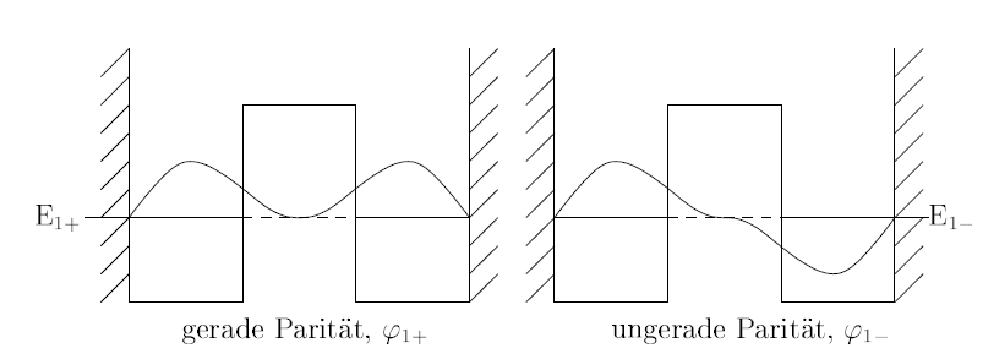
\includegraphics{./sgl_doppelmuldenpotential_pics/pic02_v.pdf}
  \caption{Symmetrische und Antisymmetrische Funktion.}
  \label{fig:fg2}
\end{figure}


Insgesamt tunnelt das Teilchen mit der Periode \(2\tau\) hin und her, d.h die Aufenthaltswahrscheinlichkeit  \(|\psi(x,t)|^2\) ergibt immer den gleichen Wert für eine zeitliche Verschiebung von \(2\tau\).


\subsubsection{Referenzen}

\begin{itemize}
\item \url{http://www.condmat.uni-oldenburg.de/Skripte/html/qm1_skript_hyper.pdf}
\end{itemize}


\end{document}

